% !TEX encoding = UTF-8 Unicode
\documentclass[a4paper]{article}

\usepackage{color}
\usepackage{url}
\usepackage[T2A]{fontenc} % enable Cyrillic fonts
\usepackage[utf8]{inputenc} % make weird characters work
\usepackage{graphicx}
\usepackage{caption}

\usepackage[english,serbian]{babel}
%\usepackage[english,serbianc]{babel} %ukljuciti babel sa ovim opcijama, umesto gornjim, ukoliko se koristi cirilica

\usepackage[unicode]{hyperref}
\hypersetup{colorlinks,citecolor=green,filecolor=green,linkcolor=blue,urlcolor=blue}

\usepackage{listings}
\renewcommand{\lstlistingname}{Kod} %da ne bi pisalo Listing 1

%\newtheorem{primer}{Пример}[section] %ćirilični primer
\newtheorem{primer}{Primer}[section]

\definecolor{mygreen}{rgb}{0,0.6,0}
\definecolor{mygray}{rgb}{0.5,0.5,0.5}
\definecolor{mymauve}{rgb}{0.58,0,0.82}

\lstset{ 
  backgroundcolor=\color{white},   % choose the background color; you must add \usepackage{color} or \usepackage{xcolor}; should come as last argument
  basicstyle=\scriptsize\ttfamily,        % the size of the fonts that are used for the code
  breakatwhitespace=false,         % sets if automatic breaks should only happen at whitespace
  breaklines=true,                 % sets automatic line breaking
  captionpos=b,                    % sets the caption-position to bottom
  commentstyle=\color{mygreen},    % comment style
  deletekeywords={...},            % if you want to delete keywords from the given language
  escapeinside={\%*}{*)},          % if you want to add LaTeX within your code
  extendedchars=true,              % lets you use non-ASCII characters; for 8-bits encodings only, does not work with UTF-8
  firstnumber=1,                % start line enumeration with line 1000
  frame=single,	                   % adds a frame around the code
  keepspaces=true,                 % keeps spaces in text, useful for keeping indentation of code (possibly needs columns=flexible)
  keywordstyle=\color{blue},       % keyword style
  language=Python,                 % the language of the code
  morekeywords={*,...},            % if you want to add more keywords to the set
  numbers=left,                    % where to put the line-numbers; possible values are (none, left, right)
  numbersep=5pt,                   % how far the line-numbers are from the code
  numberstyle=\tiny\color{mygray}, % the style that is used for the line-numbers
  rulecolor=\color{black},         % if not set, the frame-color may be changed on line-breaks within not-black text (e.g. comments (green here))
  showspaces=false,                % show spaces everywhere adding particular underscores; it overrides 'showstringspaces'
  showstringspaces=false,          % underline spaces within strings only
  showtabs=false,                  % show tabs within strings adding particular underscores
  stepnumber=1,                    % the step between two line-numbers. If it's 1, each line will be numbered
  stringstyle=\color{mymauve},     % string literal style
  tabsize=2,	                   % sets default tabsize to 2 spaces
  title=\lstname                   % show the filename of files included with \lstinputlisting; also try caption instead of title
}

\begin{document}
\title{Detekcija zajednica u socijalnim mrežama\\ \small{Seminarski rad u okviru kursa\\Računarska inteligencija\\ Matematički fakultet}}

\author{Aleksandra Nikšić, Anđelka Milovanović\\ mi16072@alas.matf.bg.ac.rs, mi15145@alas.matf.bg.ac.rs}

%\date{9.~april 2015.}

\maketitle

\abstract{
Ovaj rad se bavi metodama detekcije zajednica u socijalnim mrežama. Istraživanje je odrađeno sa Girvan-Newman algoritmom sa običnom i gustinskom modularnošću, kao i sa Meme-Net algoritmom i njegovom modifikacijom sa heuristikom simuliranog kaljenja umesto lokalne pretrage. Zajednice su bile poznati skupovi podataka: Karate, Delfini i Jazz.}

\tableofcontents

\newpage

\section{Uvod}
\label{sec:uvod}
Otkrivanje zajednica \cite{fortunato2010community} je važno istraživačko polje u analizi socijalnih mreža gde se bavimo uočavanjem strukture mreže. Struktura zajednice je ključna topološka karakteristika kompleksnih mreža. Savremena nauka o mrežama donela je značajan napredak našem razumevanju ovih složenih sistema.

Problem predstavlja uočavanje jače i slabije povezanih delova mreže na osnovu posmatranja isključivo eksplicitnih veza između čvorova. Grupe čvorova unutar kojih su mrežne veze guste predstavljaju zajednice, dok su veze između takvih grupa niže gustine. Ovakve zajednice mogu se smatrati prilično nezavisnim komponentama grafa, igrajući sličnu ulogu poput tkiva ili organa u ljudskom telu. Sposobnost pronalaženja i analiziranja takvih grupa može značajno doprineti razumevanju i vizualizaciji strukture mreža.

Detekcija zajednica nalazi veliku primenu u naukama poput sociologije, biologije ili računarstva, disciplinama u kojima su sistemi često predstavljeni kao grafovi. Primenom algritama detekcije na realne mreže možemo zaključiti osobine i veze između čvorova, koje nisu dostupne iz direktnog posmatranja grafa. 

\section{Algoritmi}
\label{sec:algoritmi}
Jednostavan način identifikovanja zajednica na grafu je detektovanje grana koje povezuju čvorove različitih zajednica i njihovo uklanjanje, kako bi se klasteri razdvojili \cite{newman2004finding}. Sa druge strane, zajednice se mogu tražiti genetskim algoritmom gde su jedinke predtavljene kao nizovi čvorova sa određenim pripadnostima. U naredne dve sekcije biće predstavljeni ovi algoritmi, jer su oni korišćeni za analizu detekcija zajednica.

\subsection{Girvan-Newman}
Algoritam koji je obeležio početak nove ere na polju detekcije zajednica predložen je od strane naučnika Girvana i Newmana \cite{newman2004finding}. U njemu se grane biraju u odnosu na vrednost njihovog centraliteta (eng. \textit{edge centrality}), koja procenjuje važnost grane. Koraci algoritma implementirani od strane Jahanbakhsh \cite{gn_algo} su sledeći:
\begin{enumerate}
\item postavi se najbolja modularnost na BestQ=0
\item učita se graf i izračunaju se njegove komponente
\item izračuna se edge-betweenness za sve ivice i obrišu se sve one sa maksimalnom vrednošću (one su most između zajednica)
\item izračuna se novi broj komponenti grafa
\item ako je novi broj komponenti $\leq$ od početnog onda se ponavlja korak 3
\item izračuna se modularnost i sačuva se u Q
\item ako je Q>BestQ onda se ažurira najbolja modularnost i sačuva se ta podela grafa kao najbolja u BestComps 
\item ako nema više ivica u grafu vraća se BestComps, u suprotnom se ponavlja proces od koraka 3 na dalje
\end{enumerate}

Fokus algoritma je na koceptu međusobnosti (eng. \textit{betweenness}), promenljivoj koja izražava frekvenciju učešća grane u procesu. Složenost izračunavanja ove promenljive je O(mn), a na retkim grafovima O($n^2$). Razmatrane su tri različite vrste, a ona koja je eksperimentalno dala najbolje rezultate je EB (eng. \textit{edge betweenness}). Ona govori koliko najkraćih putanja između svih parova čvorova na grafu u svom skupu grana sadrži baš posmatranu granu. Intuitivno je da grane unutar zajednice imaju veliku vrednost EB, zato što će dosta najkraćih putanja koje povezuju čvorove različitih zajednica preći preko njih. 

Ipak, algoritam je prilično spor i primenljiv na retke grafove sa do 10000 čvorova. Originalni algoritam nije imao proceduru za biranje najbolje particije, ali se usavršavanjem došlo se načina odabira. Particija koja će biti odabrana ima najveću vrednost modularnosti (eng. \textit{modularity}), kriterijuma koji se od tada frekventno koristi. 

Girvan Newman modularnost Q, prvobitno je uvedena radi definisanja kriterijuma zaustavljanja za algoritam Girvana i Newmana, brzo je postala suštinski element mnogih metoda za detekciju zajednica. Ona je dosta korišćena funkcija kvaliteta.

Pretpostavimo da visoke vrednosti modularnosti ukazuju dobre particije (nije generalno tačno). Dakle, particija koja odgovara njenoj maksimalnoj vrednosti na datom grafu treba da bude najbolja, ili barem vrlo dobra. To je glavna motivacija za maksimizaciju modularnosti. Iscrpna optimizacija Q-a je nemoguća zbog ogromnog broja načina na koje je moguće particionisati graf. Osim toga, stvarni maksimum je van domašaja, jer je nedavno dokazano da je optimizacija modularnosti NP-kompletan problem. Međutim, trenutno postoji nekoliko algoritama koji mogu pronaći poprilično dobre aproksimacije maksimuma modularnosti u razumnom vremenu.
Modularnost je definisana na sledeći način:

\begin{equation} Q = \frac{1}{2m} \sum_{ij}{}(A_{ij} - P_{ij}) \delta(C_{i}, C_{j})
\end{equation}
gde suma obuhvata sve parove čvorova, $A$ je matrica susedstva, $m$ je ukupan broj grana grafa, a $P_{ij}$ predstavlja očekivani broj grana između čvorova $i$ i $j$ u originalnom grafu i $\delta$ funkcija ima vrednost 1 ako su čvorovi $i$ i $j$ u istoj zajednici ($C_{i} = C_{j}$), a 0 inače.

Za datu particiju grafa $\omega = {V_{1}, V_{2}, ..., V_{m}}$, gde je $V_{i}$ skup čvorova podgrafa $G_{i}$ za $i = 1,...,m$, modularnost zasnovana na gustini (poznata kao D-vrednost) je definisana na sledeći način \cite{li2008quantitative}:

\begin{equation} D = \sum_{i = 1}^{m} \frac{L(V_{i},  V_{i}) - L(V_{i}, \overline V_{i})}{|V_{i}|} 
\end{equation}
gde su skupovi čvorova $V_{1}$ i $V_{2}$ disjunktni podskupovi skupa čvorova grafa $V$. Definišemo $L(V_{1}, V_{2}) = \sum_{i \in V_1, j \in V_2} A_{ij}$, $L(V_{1},  V_{1}) = \sum_{i \in V_1, j \in V_1} A_{ij}$ i $L(V_{1}, \overline V_{1}) = \sum_{i \in V_1, j \in \overline V_1} A_{ij}$, gde je  $\overline V_{1} = V - V_{1}$. 
U ovoj jednačini, svaki sabirak označava odnos između razlike unutrašnjeg i spoljašnjeg stepena podgrafa $G_{i}$ i veličine podgarafa. Što je vrednost D veća, particija je bolja. Dakle, problem detekcije zajednice se može posmatrati kao problem pronalaženja particije mreže takve da je modularnost zasnovana na gustini maksimizirana.

Ova funkcija kvaliteta se može i generalizovati \cite{gong2011memetic}:

\begin{equation} D_{\lambda} = \sum_{i = 1}^{m} \frac{2 \lambda L(V_{i},  V_{i}) - 2(1 - \lambda)L(V_{i}, \overline V_{i})}{|V_{i}|} 
\end{equation} Variranjem $\lambda$ možemo posmatrati mrežu u različitim rezolucijama. Parametar $\lambda$ može uzeti vrednost u opsegu od 0 do 1. Za veće vrednosti $\lambda$ ovaj metod ima tendenciju da zajednicu razbija na više manjih zajednica. Za manje vrednosti $\lambda$ dobija se podela na veće zajednice.

%Razvijeno je mnoštvo proširenja i modifikacija algoritma, koje su za cilj imale ubrzavanje procesa izračunavanja preko poboljšanja mere kvaliteta grana. Neke od njih su Monte Karlo varijanta ponovnog uzorkovanja koju je predlozio Tyler i varijanta bazirana brojanju kratkih ciklusa koju je predložio Radicchi.
%predlog - nabrojati razna usavrsavanja algoritma


\subsection{Memetski algoritam}
Za detekciju zajednica u okviru memetskog  algoritma \cite{gong2011memetic} optimizovaćemo modularnost zasnovanu na gustini. Razmatraćemo i podesivi parametar $\lambda$ koji nam daje mogućnost istraživanja mreže u različitim rezolucijama. Ovaj algoritam je originalno simbioza genetskog algoritma i strategije lokalne pretrage. U ovom radu heuristiku lokalne pretrage zamenićemo tehnikom simuliranog kaljenja. 

U standardnom genetskom algoritmu, populacija stringova (hromozoma), koja enkodira kandidate (jedinke) za rešenje optimizacionog problema, evoluira ka boljim rešenjima. Evolucija najčešće kreće iz nasumično izabrane populacije. U svakoj generaciji, izračunava se fitnes svake jedinke, bira se određen broj jedinki koji će učestvovati u modifikaciji (operatorima ukrštanja i mutacije) da bi oformili novu populaciju. Nakon nekoliko generacija, samo ona rešenja sa velikom vrednošću fitnesa će preživeti. U radu Gonga i drugih naučnika \cite{gong2011memetic}, modularnost je fitnes funkcija, a particije su hromozomi. Evolutivni algoritmi koji rekombinaciju viskokvalitetnih rešenja presecaju pojedinačnim optimizacijama nazvani su memetski algoritmi. Metode su inspirisane modelima prirodnih sistema koji kombinuju evolucijsku adaptaciju populacije sa individualnim učenjem tokom životnog veka njenih članova. Više o tome kako se generiše inicijalna populacija i na koji način se vrše operacije ukrštanja i mutacije jedinki pročitati u radu \cite{gong2011memetic}, a implementacioni detalji se mogu pogledati na adresi: \url{https://github.com/newxd/community-detection}.

Simulirano kaljenje iskoristićemo kako bismo poboljšali pojedinačna rešenja. Pri ažuriranju najbolje jedinke pretraživaćemo njenu okolinu i analizirati funkcije cilja datih rešenja. Ukoliko naiđemo na rešenje sa boljom vrednošću funkcije cilja, ažuriraćemo najbolje rešenje pronađenim. Ukoliko naiđemo na rešenje sa lošijom vrednošću funkcije cilja, poredićemo vrednosti unapred definisane funkcije  p  i proizvoljno izabrane vrednosti  q  iz intervala  (0,1). Ako je p > q, ažuriraćemo najbolje rešenje pronađenim.


%Ova sekcija će biti reprodukovan rad \cite{gong2011memetic} s razlikom u odabiru metaheuristike. U originalnom radu, algoritam koristi lokalnu pretragu koju smo zamenili tehnikom simuliranog kaljenja.


\section{Rezultati}	
\label{sec:rezultati}
U ovoj sekciji biće prestavljeni rezultati dobijeni nad podacima skupova Karate, Delfin i Jazz. Nad svakim skupom eksperimentisano je sa dve verzije Girvan-Newman algoritma (obična modularnost \cite{fortunato2010community} i modularnost sa gustinom \cite{li2008quantitative}), kao i sa verzijama Memetskog algoritma sa podrazumevanom lokalnom pretragom (Meme-Net \cite{gong2011memetic}) i sa dodatom heuristikom simuliranog kaljenja koje je isprobano sa ciljem eksperimentisanja.

\subsection{Karate skup}
Karate skup (eng. Zachary’ s karate club) se sastoji od 34 čvora i 78 ivica. Konstruisao ga je Zachary, posmatrajući 34 člana karate kluba tokom perioda od 2 godine. Nakon svađe između šefa kluba i instruktora, zajednica se podelila na 2 dela, jer je instruktor napravio svoj klub i odveo oko polovine članova \cite{gong2011memetic}. 

Gong et al. su u svom radu osmislili Meme-Net algoritam, koji je rekonstruisan u ovom radu. Dodatak tom algoritmu jeste simulirano kaljenje koje je isprobano u delovima u kojima je bilo predviđeno da se koristi lokalna pretraga. Pored eksperimentisanja sa simuliranim kaljenjem u Meme-Net algoritmu, isprobana je i verzija GN algoritma gde se za funkciju modularnosti koristi gustinska modularnost.

Na slici \ref{fig:GN1} se jasno može videti da je podela sa gustinskom modularnošću bolje podelila graf, što je potvrdila i NMI (eng. Normalized Mutual Information) veličina, koja je za običan GN bila ~0.58, dok je za izmenjenu modularnost iznosila NMI: ~0.84. Menjanjem parametara ovo se nije moglo unaprediti dalje.
\begin{figure}[h!]
\centering
\captionsetup{justification=centering,margin=1cm}
\begin{center}
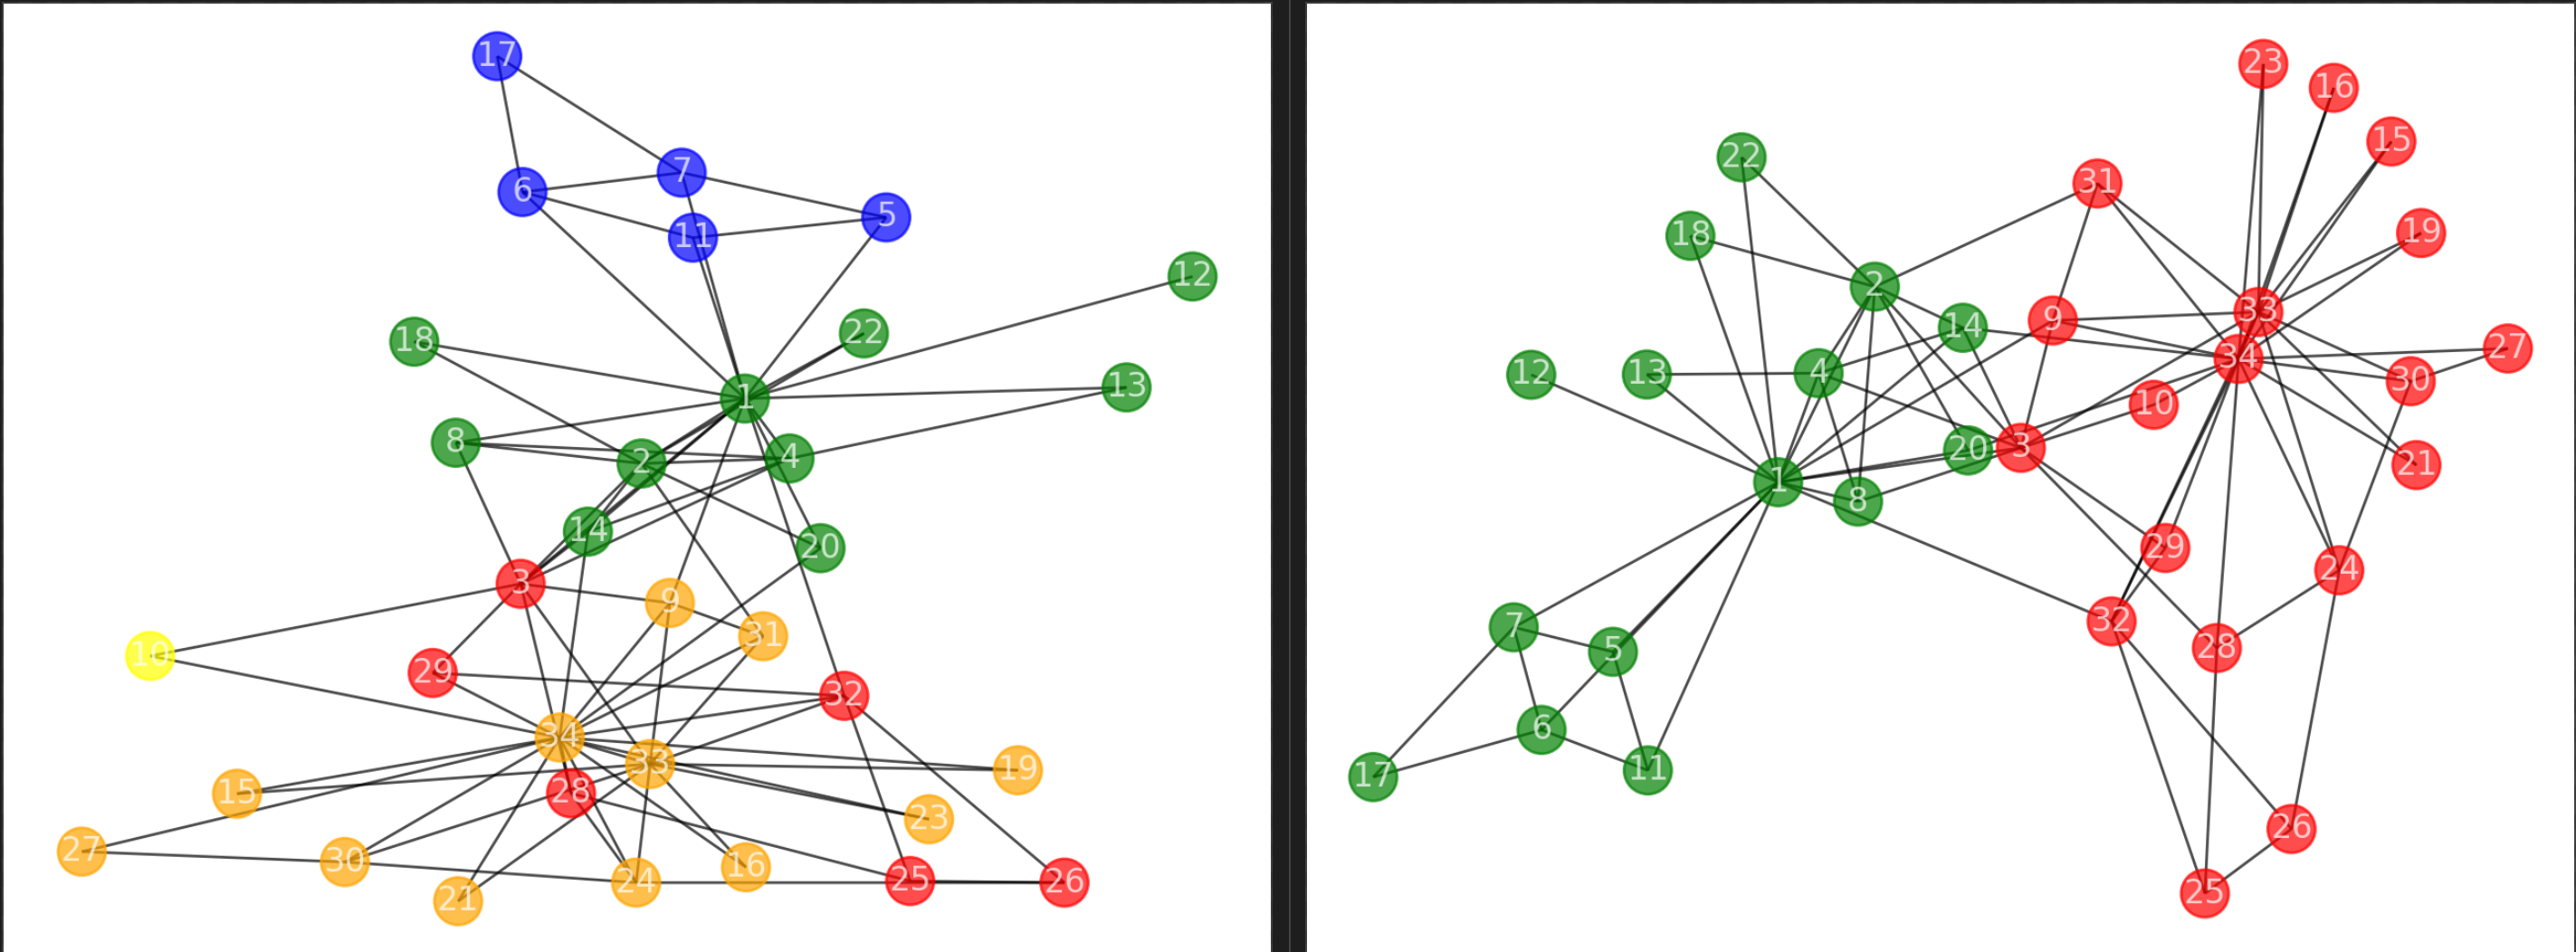
\includegraphics[scale=0.21]{seminarski_forma/Karate_GN_basic_vs_density.png}
\end{center}
\caption{Sa leve strane slike je podrazumevani GN, dok je sa desne strane GN sa gustinskom modularnošću sa parametrom $\lambda$=0.3}
\label{fig:GN1}
\end{figure}
Na slici \ref{fig:Meme1} su predstavljeni rezultati dobijeni pokretanjem Meme-Net algoritma za 20 generacija i $\lambda$=0.5. Sa leve strane je Meme-Net, a sa desne strane izmenjena verzija sa simuliranim kaljenjem od 500 iteracija. NMI vrednosti su bile redom: ~0.22 i ~0.7.
\begin{figure}[h!]
\centering
\captionsetup{justification=centering,margin=1cm}
\begin{center}
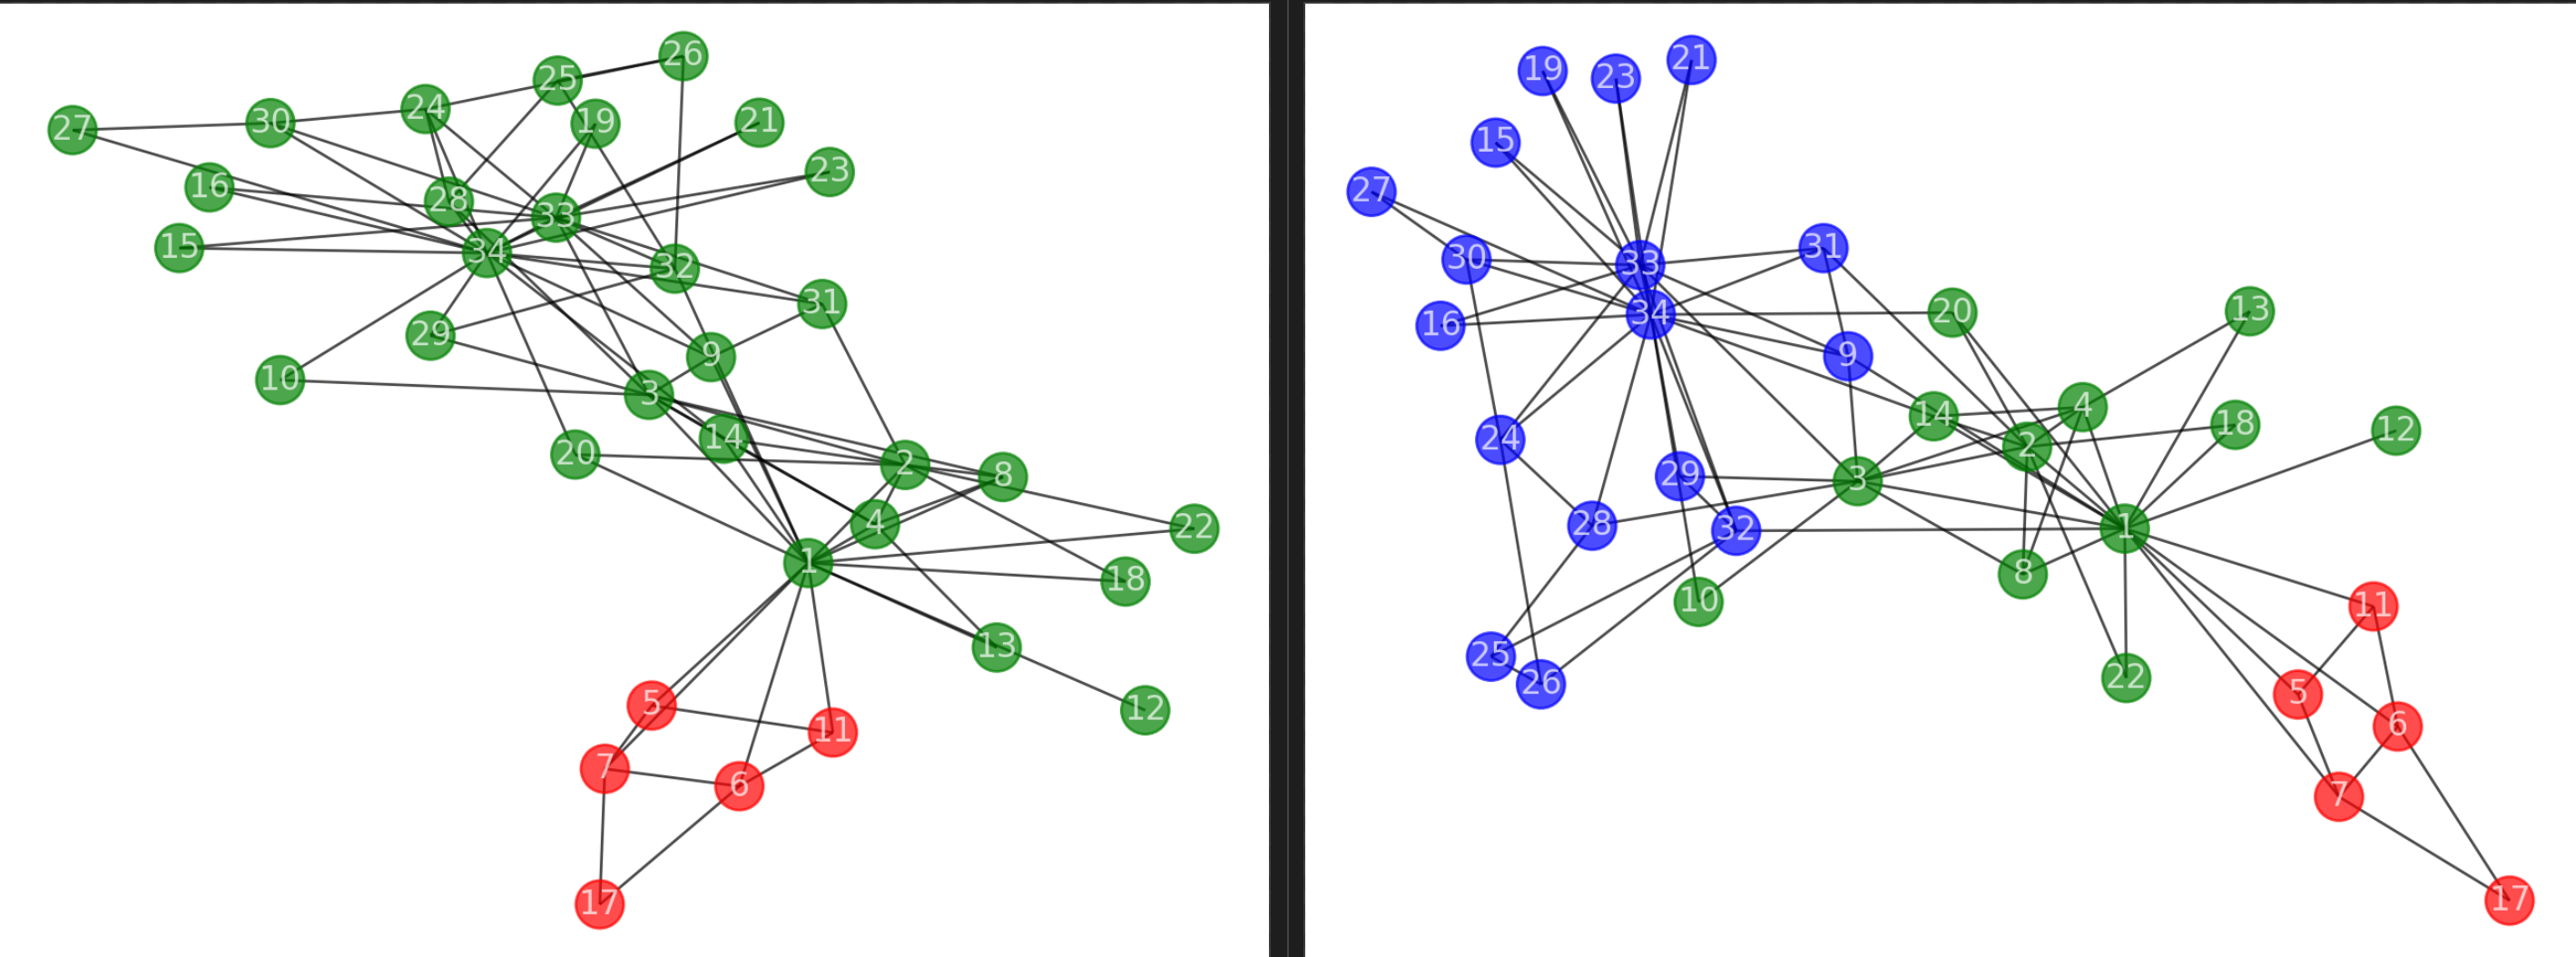
\includegraphics[scale=0.21]{seminarski_forma/Karate_MA_Local_vs_SAnnealing_20_generations.png}
\end{center}
\caption{Sa leve strane slike je Meme-Net, dok je sa desne strane Meme-Net sa simuliranim kaljenjem (oba za 20 generacija) i $\lambda$=0.5}
\label{fig:Meme1}
\end{figure}
Kada se $\lambda$ parametar postavi na 0.3 vrednost (predloženu u \cite{gong2011memetic}), dobija se NMI=1 sa simuliranim kaljenjem za 20 generacija, dok običan Meme-Net ima značajno manju NMI nakon toliko generacija. Rezultati su predstavljeni na slici \ref{fig:Meme2}.
\begin{figure}[h!]
\centering
\captionsetup{justification=centering,margin=1cm}
\begin{center}
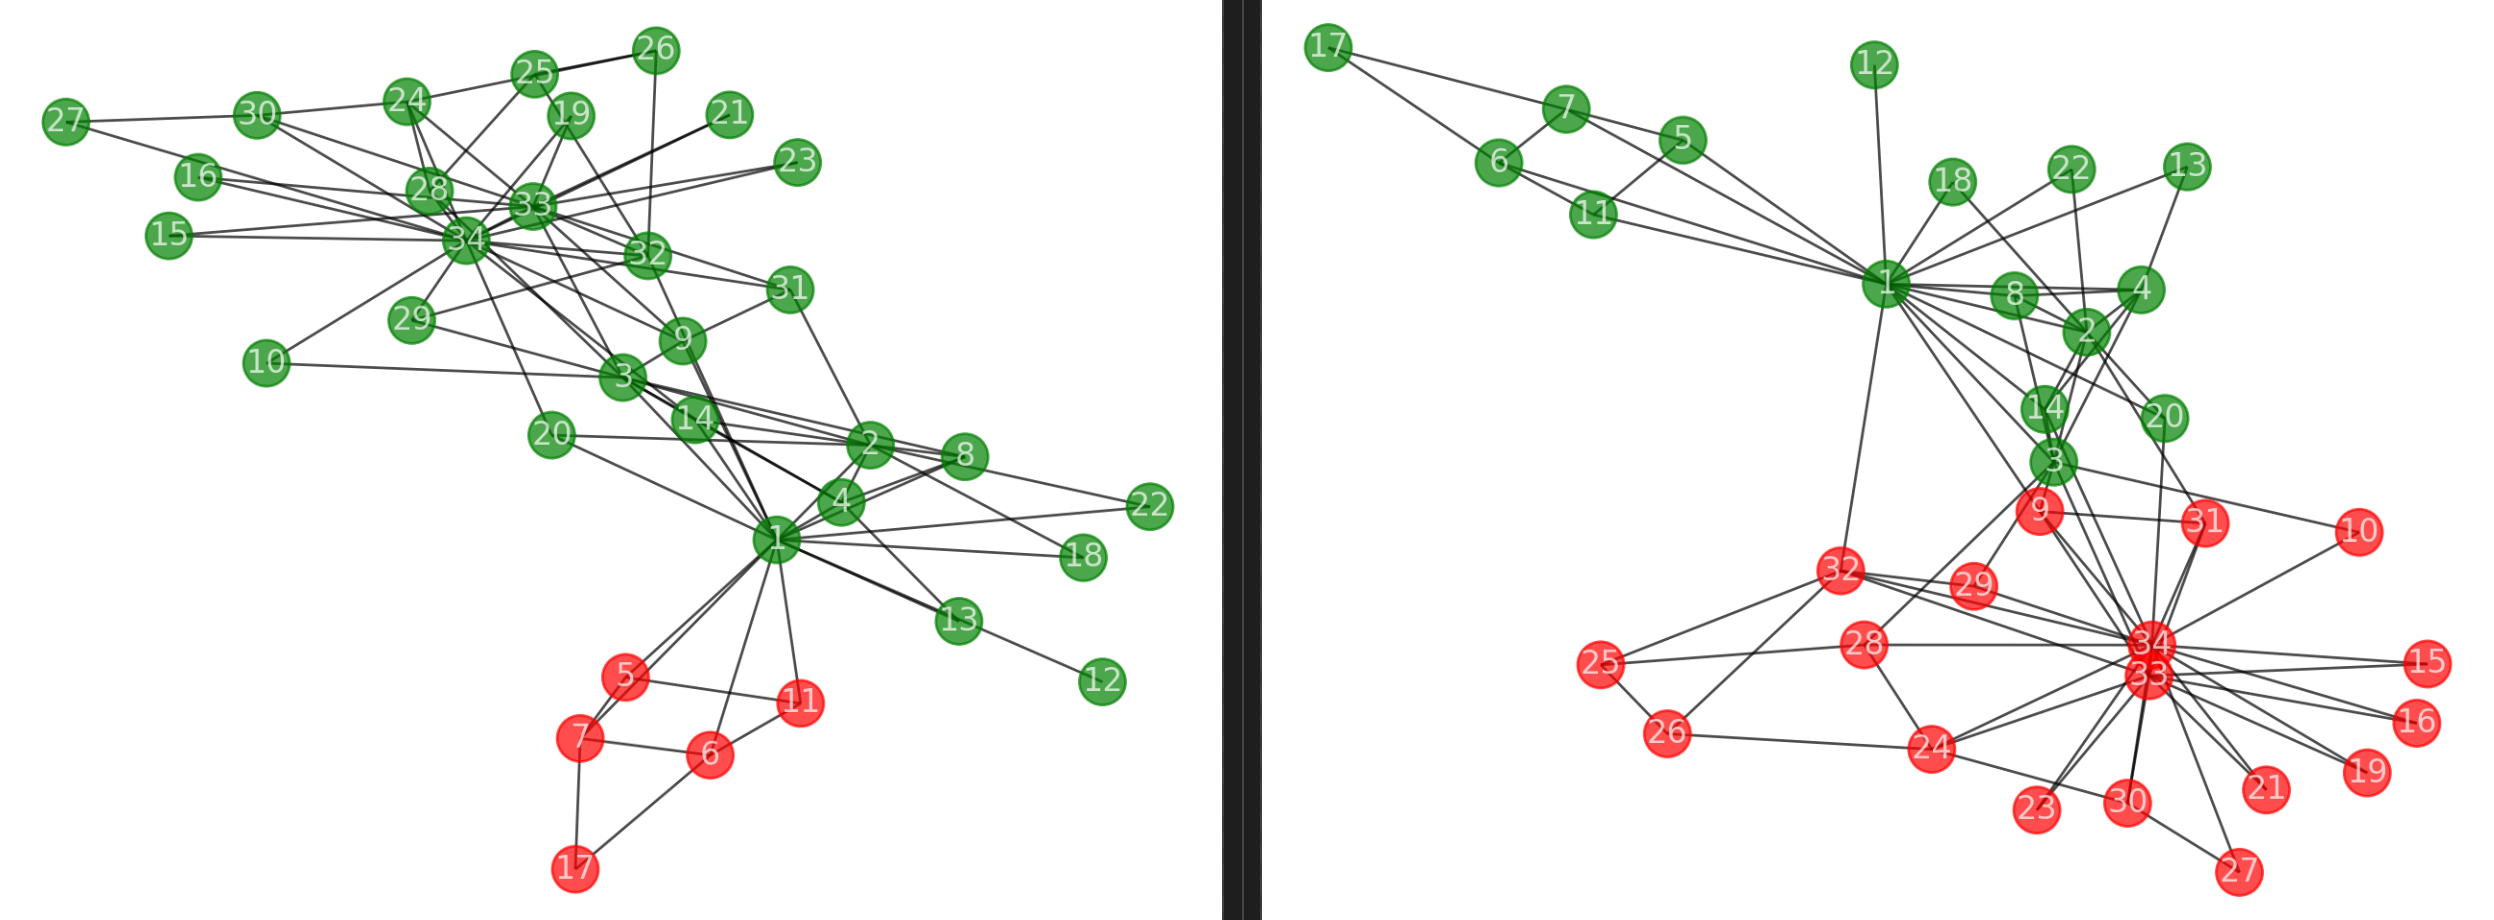
\includegraphics[scale=0.23]{seminarski_forma/GN3_comparing.png}
\end{center}
\caption{Sa leve strane slike je Meme-Net, dok je sa desne strane Meme-Net sa simuliranim kaljenjem (oba za 20 generacija) i $\lambda$=0.3}
\label{fig:Meme2}
\end{figure}

\subsection{Delfin skup}
Skup delfina sastoji se od 62 delfina i 159 veza između njih. Delfini su sa Novog Zelanda i podaci o njima su prikupljani tokom 7 godina. Veza tj. ivica između 2 delfina je ostvarena na osnovu njihovog statistički čestog druženja. Prirodno se mreža deli u 2 velike grupe \cite{gong2011memetic}.

Ono što se može zaključiti iz GN algoritma je kao i kod Karate skupa, da se izmenom modularnosti na gustinsku modularnost, može postići veći NMI, ali ne može dostići vrednost 1. Rezultati su prikazani na slici \ref{fig:GN_Dolp_1}. Što se tiče memetskog algoritma, nakon 50 generacija NMI dostiže vrednost 1 sa simuliranim kaljenjem, dok lokalna pretraga dostiže vrednost ~0.48. Rezultati su prikazani na slici \ref{fig:Meme_dolp1}. 

\begin{figure}[h!]
\centering
\captionsetup{justification=centering,margin=1cm}
\begin{center}
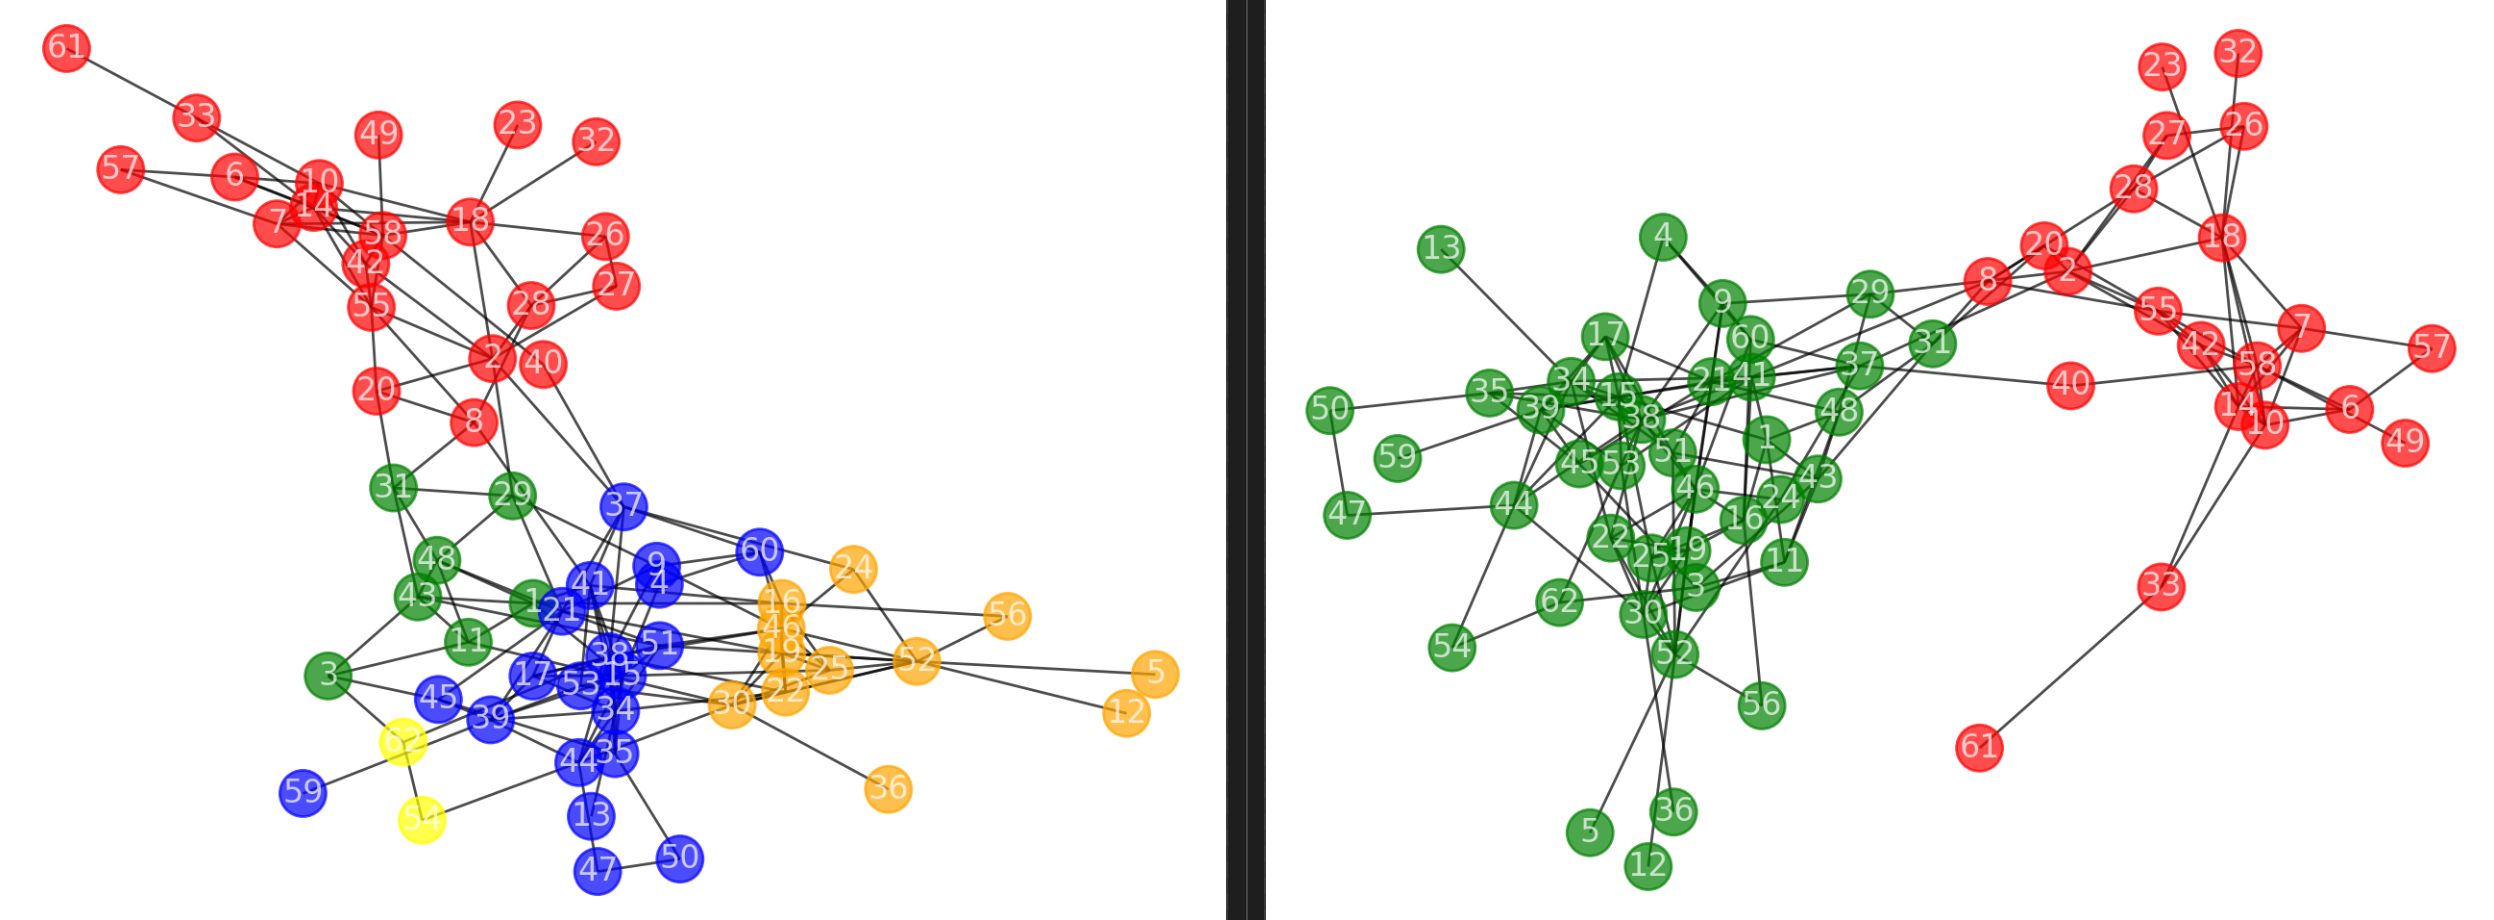
\includegraphics[scale=0.23]{seminarski_forma/GN_dolphins1.png}
\end{center}
\caption{Sa leve strane slike je podrazumevani GN, dok je sa desne strane GN sa gustinskom modularnošću sa parametrom $\lambda$=0.3.}
\label{fig:GN_Dolp_1}
\end{figure}

\begin{figure}[h!]
\centering
\captionsetup{justification=centering,margin=1cm}
\begin{center}
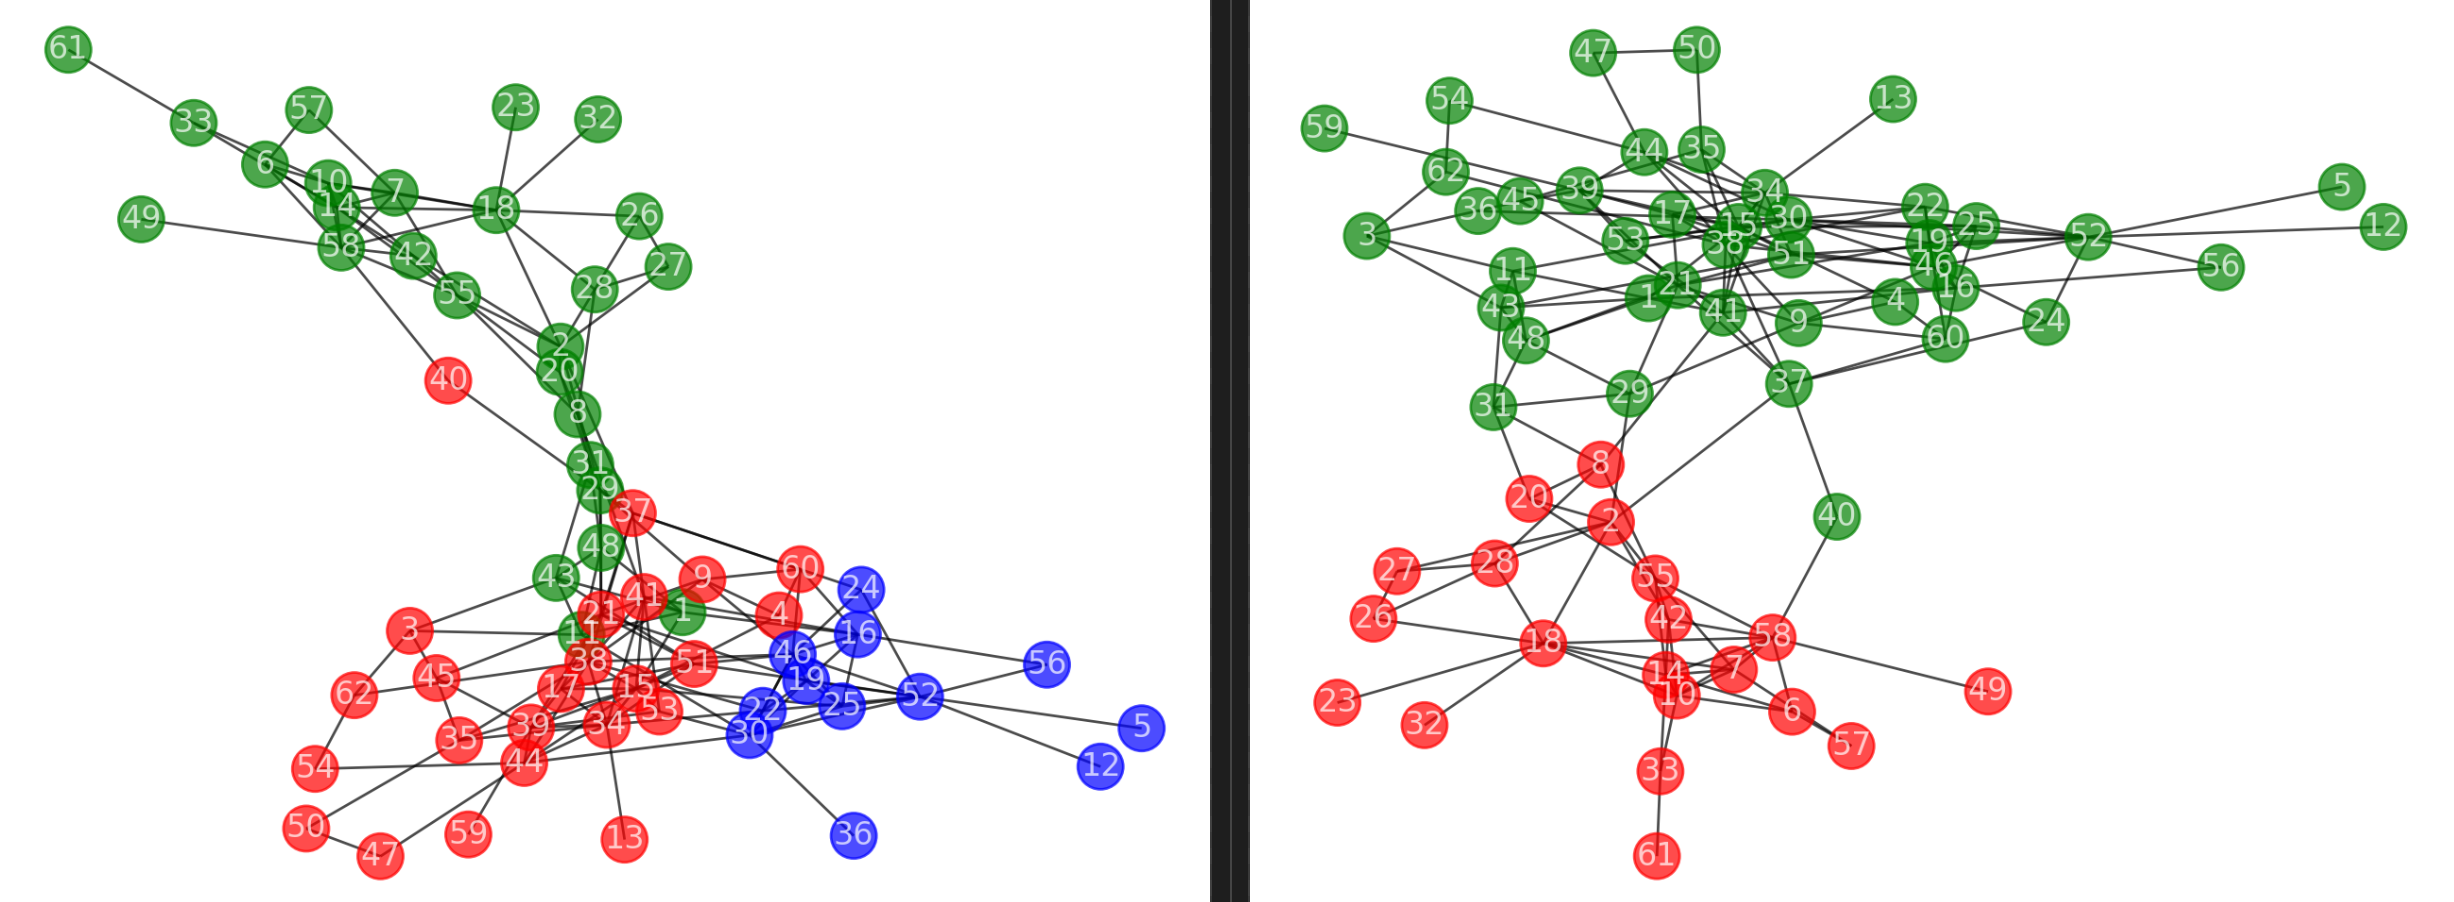
\includegraphics[scale=0.23]{seminarski_forma/MA_dolphin.png}
\end{center}
\caption{Sa leve strane slike je Meme-Net, dok je sa desne strane Meme-Net sa simuliranim kaljenjem (oba za 50 generacija) i $\lambda$=0.3}
\label{fig:Meme_dolp1}
\end{figure}

\subsection{Jazz skup}
Jazz skup predstavlja mrežu muzičara. Ukupan broj čvorova je 198 i svaki čvor predstavlja jednog muzičara. Broj ivica je 5484 i ivica između muzičara postoji ukoliko su 2 muzičara bili članovi istog benda. Podaci su sakupljeni tokom 2003. godine \cite{konect:2016:arenas-jazz}.

Izveštaj sa informacijama za ovaj skup biće predstavljen na odbrani seminarskog rada.

\newpage

\section{Zaključak}
\label{sec:zakljucak}
Tokom istraživanja oblasti detekcije zajednica u socijalnim mrežama, zaključeno je da se u zavisnosti od problema različiti algoritmi ponašaju bolje ili lošije. Naš rad je ograničen na istraživanje Girvan-Newman algoritma, kao i memetskog algoritma.

Rezultati su pokazali da se izmenom klasične modularnosti sa gustinskom modularnošću kod algoritma Girvan-Newman dobijaju značajno bolje particije grafa. To je utvrđeno poređenjem sa stvarnom particijom skupova Karate i Delfin, koristeći NMI meru. 

Što se tiče izmene u Meme-Net algoritmu u kome smo umesto lokalne pretrage primenili heuristiku simuliranog kaljenja, ne može se sa sigurnošću reći da uvek radi brže i bolje. Međutim, za ispitane slučajeve konvergencija je bila brža i NMI je dostizao vrednost 1.

Dalji rad bi mogao da se fokusira na istraživanje većih zajednica ovim algoritmima.

\addcontentsline{toc}{section}{Literatura}
\appendix
\bibliography{seminarski} 
\bibliographystyle{plain}

\appendix
\section{Dodatak}
GitHub repozitorijum seminarskog rada se može naći na adresi: \url{https://github.com/mandja96/RI-detekcija_zajednica}.
\end{document}